\documentclass[a4paper,10pt, fleqn]{article}
%\documentclass[a4paper,10pt]{scrartcl}

\usepackage[utf8]{inputenc}
\usepackage{amsmath,amssymb,amstext}
\usepackage{geometry}
\usepackage{fancyhdr}
\usepackage{listings}
\usepackage{color}
\usepackage{array, graphicx}

\begin{document}

\section{Fehler}
\label{sec:fehler}


Gaußkurve: $H(x) = \frac{1}{\sqrt{2\pi\sigma^{2}}}e^{-\frac{(x-x_{0})^{2}}{2\sigma^{2}}}$

...

\section{Geschwindigkeit}
\label{sec:geschwindigkeit}
\begin{itemize}
\item $v(t) = \frac{dx(t)}{dt}$
\item $a(t) = \frac{dv(t)}{dt} = \frac{d^{2}x}{dt^{2}}$
\item Winkel $\alpha$
  von Tangente an Funktion: $\tan\alpha = \frac{df(x)}{dx}$

\item Ableitungsregeln, Extremaregeln...
\end{itemize}

\section{Drehbewegung}
\label{sec:drehbewegung}
\begin{itemize}
\item Winkelgeschwindigkeit: $\omega = \frac{d\phi}{dt}$, $[\omega] = s^{-1}$
\item Periode $T = \frac{2\pi}{\omega_{0}}$
\item Drehfrequenz: $\nu = \frac{1}{T} = \frac{\omega_0}{2\pi}$
\item Umfangsgeschwindigkeit: $v_{Umf} = \frac{2\pi R}{T} = 2\pi R\nu = R \omega_0$
\item Vektoren: Rechenregeln, ...
\item $v = v_0 + \int_0^ta(t')dt'$
\item $r = r_0 + \int_0^tv(t')dt'$
\item $v_{0,x} = v_0\cos \phi, v_{0, z} = v_0 \sin \phi$
\item Beschleunigung:

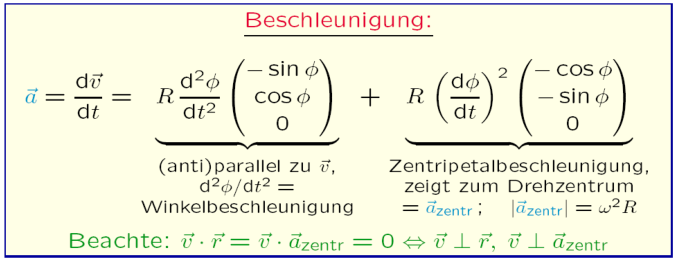
\includegraphics[width=10cm]{Beschleunigung}
\item $\vec{v} = \vec{\omega} \times \vec{r}$
\end{itemize}

\section{Kraft und Masse}
\label{sec:kraft-und-masse}

\begin{itemize}
\item $\vec{G} = m\vec{g}$
\item Elastische Verformungen: $\vec{F} = -D\vec{x}$, $D$: Federkonstante
\item Haftreibung: $|\vec{F}_H| = \mu_H |\vec{F}_N|$
\item Gleitreibung: $|\vec{F}_G| = \mu_G |\vec{F}_N|$, $\mu_G < \mu_H$
\item Rollreibung: $|\vec{F}_R| = \mu_R |\vec{F}_N|$ ???
\item Gravitationskraft der Erde: $\vec{F}(\vec{r}) = -G\frac{mM_E}{r^2} \frac{\vec{r}}{|\vec{r}|}$
\item Newtonsche Gesetze...
\item Kraft erzeugt Impulsänderung: $\Delta \vec{p} = \int_{t_1}^{t_2}\vec{F}(t)dt$
\item Umgekehrt: $\frac{d\vec{p}}{dt} = \vec{F}_{ext}$
\item Impulserhaltung...
\item $W = \int_{x_1}^{x_2}F(s)ds$
\item Potentielle Energie im Erd-Gravitationsfeld: $E_P(r) = -\frac{GmM_E}{r}$
\item $E_{kin} = \frac{1}{2}mv^2$
\item Schiefe Ebene: $mgh = \frac{1}{2}mv^2 \Rightarrow v = \sqrt{2gh}$
\item Leistung: $P = \frac{dW}{dt}$
\item $P = \vec{F} \cdot \vec{v}$
\item Stöße...
\end{itemize}

\section{Drehung}
\label{sec:drehung}

\begin{itemize}
\item Corioliskraft: $a_c = 2v\omega$, $F_c = 2m (\vec{v} \times \vec{\omega})$
\item Zentrifugalkraft...
\item Drehimpuls: $\vec{r} \times \vec{p}$

  $\Rightarrow$ Erhaltungsgröße in abgeschlossenen Systemen, ändert sich nur, wenn Drehmoment angreift.
\item Drehmoment: $\vec{D} = \frac{d\vec{L}}{dt} = \vec{r} \times \vec{F}$
\item Trägeitsmoment: Bei Drehung um Symmetrieachse: $\vec{L} = \mathbf{I}\vec{\omega}$
\item Steinerscher Satz:

  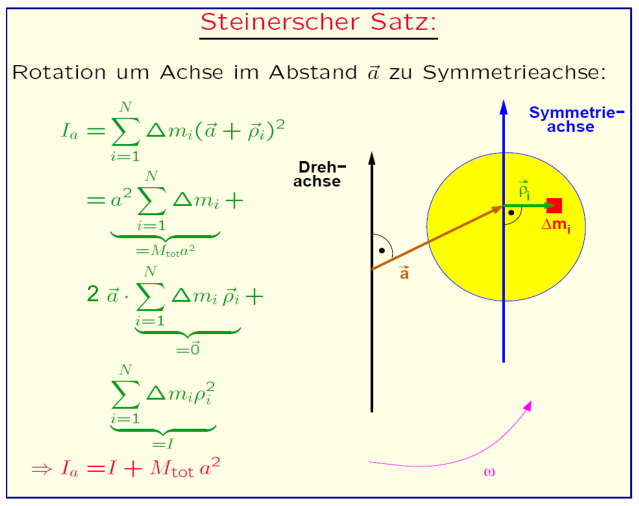
\includegraphics[width=10cm]{SteinerscherSatz}
\item Bei Rotation um feste Drehachse: $E_{rot/kin} = \frac{1}{2}I\omega^2 = \frac{L^2}{2I}$
\item Vergleich Translation $\Leftrightarrow$ Rotation:

  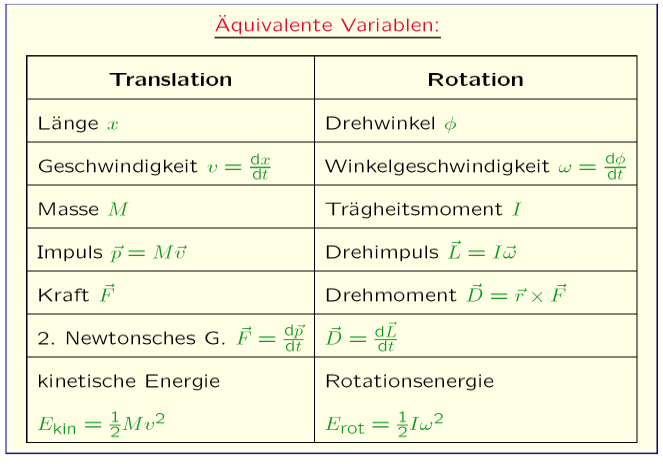
\includegraphics[width=10cm]{TranslationVsRotation}
\item Kreisel: $E_{rot} = \frac{1}{2}\vec{L}\vec{\omega}$
\item mehr Kreisel...
\end{itemize}

\section{Planetenbahnen}
\label{sec:planetenbahnen}

\begin{itemize}
\item Keplersche Gesetze:

  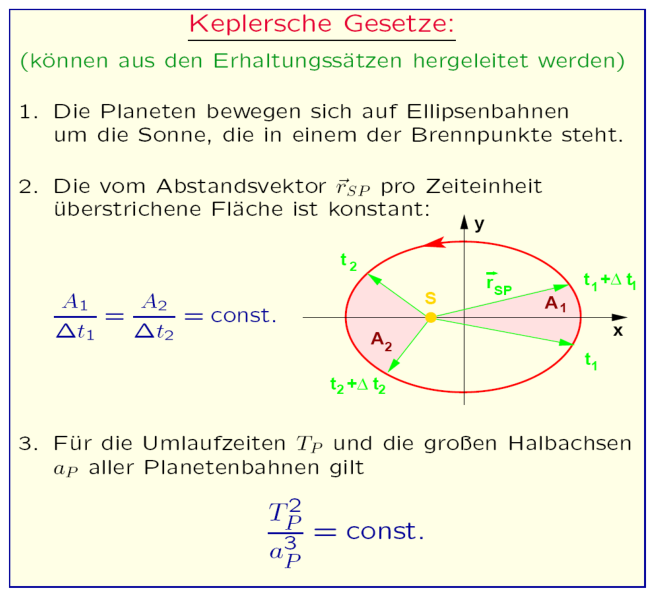
\includegraphics[width=10cm]{KeplerscheGesetze}
\end{itemize}

\section{Schwingung}
\label{sec:schwingung}

\begin{itemize}
\item Federpendel: $\ddot{x} = -\frac{D}{M}x$
\item Lösung der Schwingungsgleichung:

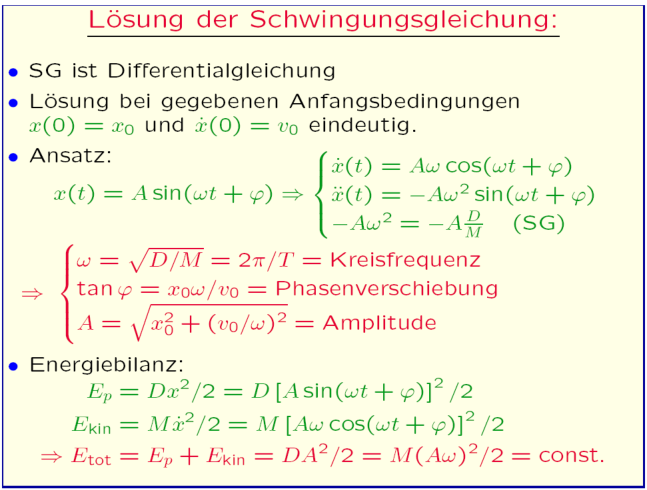
\includegraphics[width=10cm]{Schwingungsgleichung}
\item Andere Schwingungen...
\end{itemize}

\section{Wellen}
\label{sec:wellen}

\begin{itemize}
\item konstante Ausbreitungsgeschwindigkeit: $v = $ const.
\item Wellengleichung: $\frac{\partial^2\xi}{\partial z^2} = \frac{1}{v^2} \frac{\partial^2 \xi}{\partial t^2}$
\item Wellenlänge: $\lambda = Tv = \frac{2\pi}{\omega} v = \frac{v}{\nu}$
\item Wellenzahl: $k = \frac{2\pi}{\lambda} = \frac{\omega}{v}$
\item Harmonische Welle:

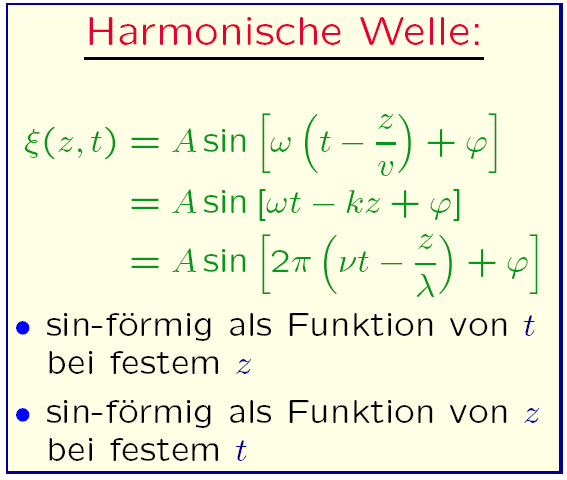
\includegraphics[width=5cm]{HarmonischeWelle}
\item Transversale vs. Longitudinale Welle...
\item Konstruktive und destruktive Interferenz:

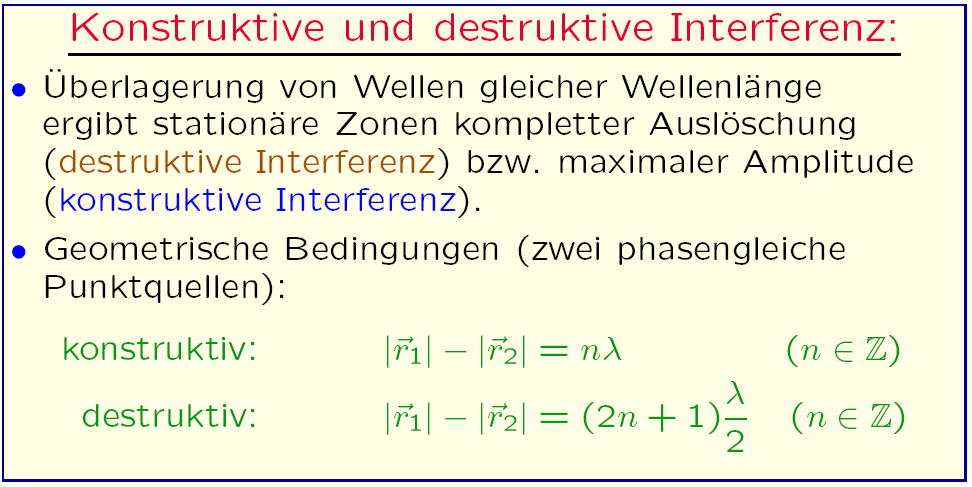
\includegraphics[width=10cm]{Interferenz}
\item Welle gegen Wand (Reflexion):

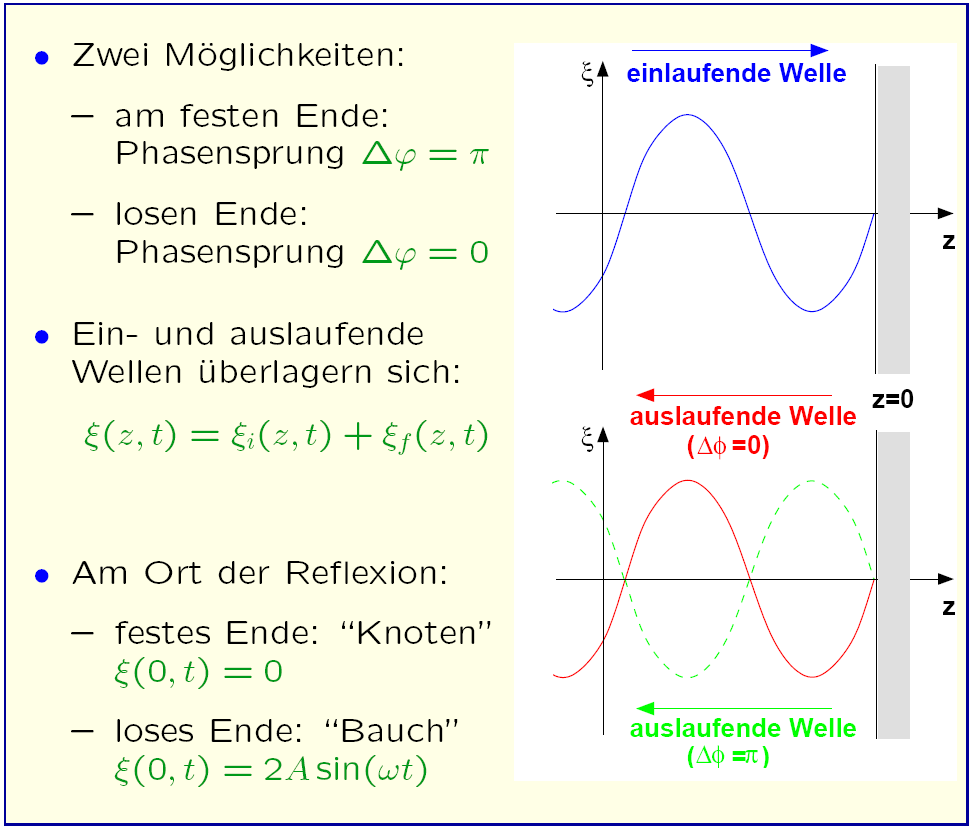
\includegraphics[width=10cm]{WelleGegenWand}
\item Stehende Welle: Immer selber Punkt von Welle an einem Ort, aber variable Amplitude.
\item Normale Welle: Überall gleiche Amplitude, aber räumlich variierende Phase
\item Resonanz:

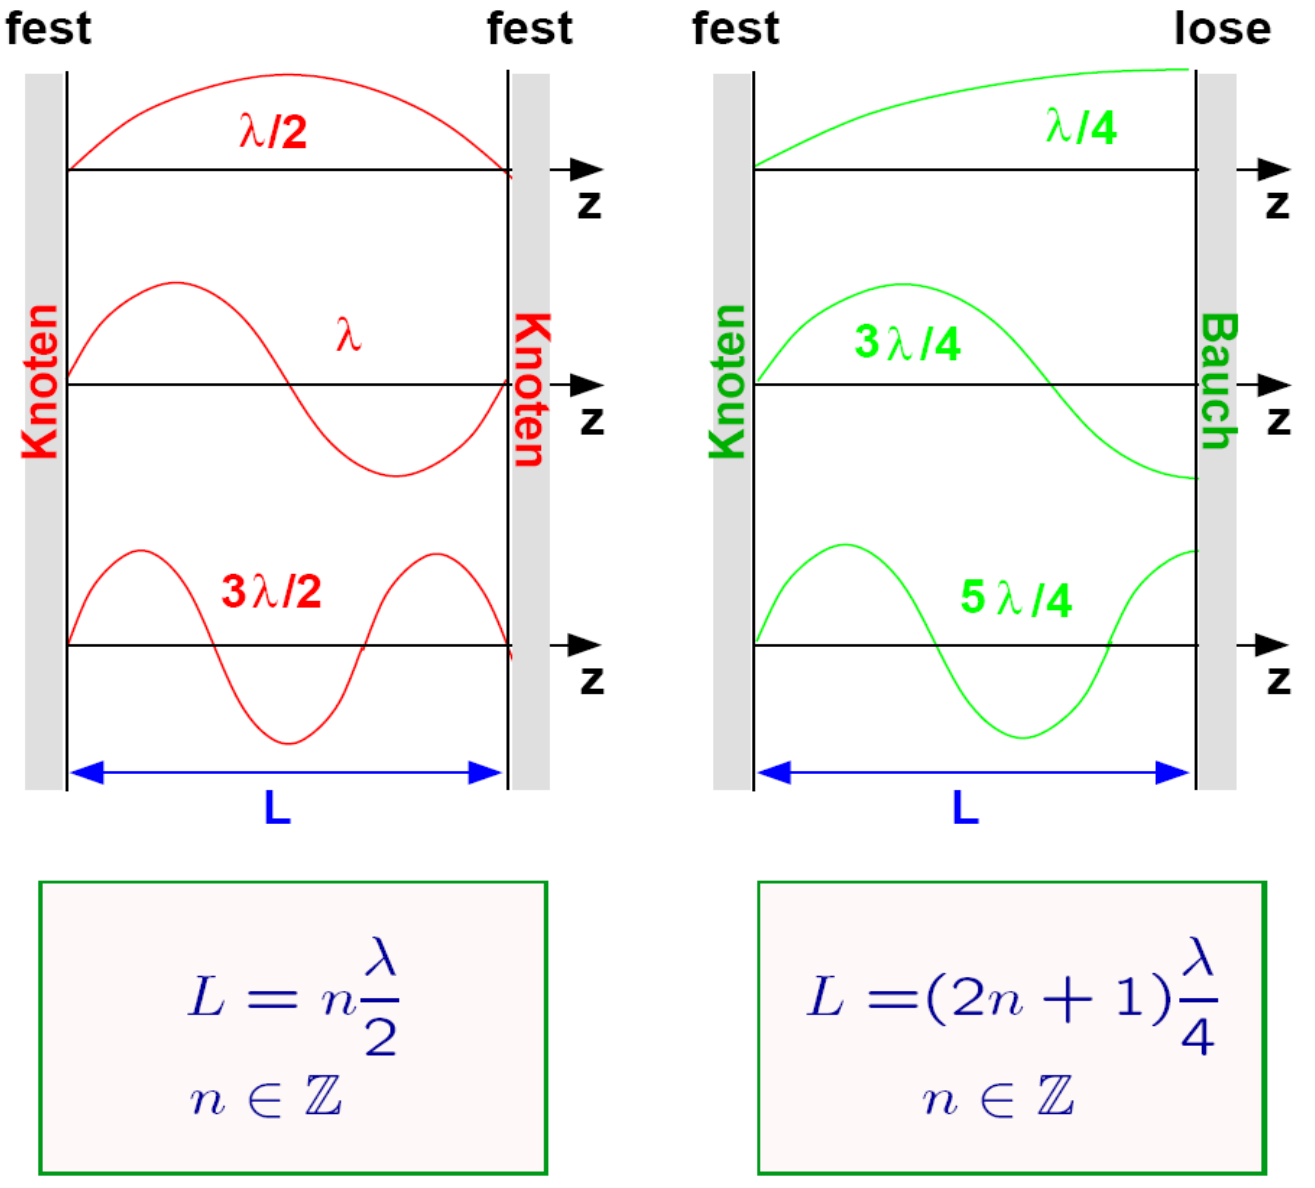
\includegraphics[width=10cm]{Resonanz}
\end{itemize}
\end{document}

%%% Local Variables:
%%% mode: latex
%%% TeX-master: t
%%% End:
